
\section{Generalized taxonomy similarity}

We now turn to a general case when one string can match multiple nodes in the taxonomy tree. In this section,  we first describe three key properties that a new function should guarantee and then we describe a new similarity function and the corresponding algorithm.



\subsection{Properties for new functions}

We define a new similarity function, which has the following three properties, called the three C's features:

(1) \textbf{Constructive }:  The new similarity is always greater than the one without considering the taxonomy. That is, using taxonomy  cannot decrease the similarity between strings in all cases; $f(S,T,\mathcal{T} ) \geq  f(S,T) $

(2) \textbf{Compatible}. When the taxonomy is updated with the insertion of the elements, the similarity always increases. That is, the similarity is upward compatible; $f(S,T,\mathcal{T} ) \leq  f(S,T, \mathcal{T'}) $ if $\mathcal{T}$ contains more elements than $\mathcal{T'}$.

(3) \textbf{Consistent}, Given two sets of tokens: S=\{$s_1,s_2,...s_n$\} and T=\{$t_1,t_2,...,t_m$\}, the maxim TS similarity between $s_i$ and $t_j$ is max, and the minimum is min. Then $ min \leq f(S,T,\mathcal{T} ) \leq max $. That means, the final similarity is consistent with the similarity of two single elements.

\subsection{Generalized taxonomy functions}


\begin{definition} [Weight functions] Given two strings $S_1$ and $S_2$ and a taxonomy $T$, the weight function w: $S \times T \rightarrow R$ is defined by $w(s_i, t_j,T)$ = $TS(s_i,t_j,T)$, where $s_i \in S$ and $t_j \in T$.
\end{definition}

\begin{definition} [Maximum Similarity Matching] Given two strings $S$ and $T$ and a taxonomy $\tau$, the weight function w: $S \times T \rightarrow R$, find a matching of maximum weight $W$ where the weight of matching $M$ is given by $w(M)$ = $\Sigma_{e \in M} w(e)$.
\end{definition}

\begin{definition} [Extended taxonomy similarity] Given two strings $S$ and $T$ and a taxonomy $\tau$, the similarity is   $\frac{W(S,T,\tau)}{max(|S_1|,|S_2|)}$, where $W(S,T,\tau)$ denotes that the value of the maximum weight matching.  \label{def:efs}
\end{definition}

\smallskip

\begin{lem}  The ETS function is constructive, compatible and consistent.
\end{lem}
\begin{proof} Because the answer is based on the maximum weighted function so the constructive and compatible is easy to prove. In order to prove the consistent.
\end{proof}

The maximum  similarity  matching is computed by the maximum weight matching in bipartite graphs. The weight is calculated by the binary similarity of any two elements.

The algorithm of the maximum weight matching in bipartite graphs is called the Hungarian method. The time analysis of the algorithm is $O(n^3)$.


Therefore, the  time analysis for the overall cost to compute two strings is $O(n^3+m^2)$, where $m$ is the sum of the length of prefix labels of words in two strings.





\subsection{String similarity join algorithms}


\begin{figure}[t]
\centering
\includegraphics[scale=0.4]{figures/sketch01}
 \caption{Illustration to FM sketches }
\label{fig:similaritygeaph}
\end{figure}


\begin{figure}
\centering
\includegraphics[scale=0.4]{figures/sketch02}
 \caption{Illustration to Bit-min sketches }
\label{fig:similaritygeaph}
\end{figure}

A naive algorithm to compute similarity join is the nested loop join to compare every pair of records. This method is obviously prohibitively expensive for large data sets. Efficient algorithms exists by following the ``filtering and verification'' framework, that is,given two collections of strings, one or multiple filters are utilized to prune away many record pairs and then the verification is involved for the remaining pairs after filtering. Clearly, the stronger filtering power, the better performance of the algorithm, because the computation of similarity between two sets are really expensive by the Hungarian algorithm. We develop two filters as follows.

\begin{lem} [\textbf{Length filter}] Given two sets of tokens $S$ and $T$ and a threshold $\theta$, without loss of the generality, assume that $|S| < |T|$,  if $ETS(S,T) > \theta$. then $|S|> \theta |T|$,

\end{lem}

\smallskip

\begin{lem} [\textbf{Similarity filter}] Given two sets $S$ and $T$. If $ETS(S,T) > \theta$, without the loss of generality, assume that $|S|<|T|$. If $ETS(S,T) > \theta$,  then there are at least $p$ distinct pairs of elements ($s_i, t_j$) in  $S$ and $T$ such that each $TS(s_i, t_j) > \frac{\theta |T| - p +1}{|S|-p+1} $. \label{lem:pthreshold}
\end{lem}

\smallskip



\begin{algorithm}
{\bf Input}: two collections of strings $S_1$ and $S_2$,  a threshold $\theta$ \\
{\bf Output}: string pairs $(s_1,s_2) \in S_1 \times S_2$, s.t. $TS(s_1, s_2) > \theta$
\begin{compactenum}[(1)]
\item Let $T_1$ and $T_2$ denote two LS tree for $S_1$ and $S_2$ respectively.
\item Initialize two cursors in two tries.
\item {\bf WHILE} $\neg end(T_s) \wedge  \neg end(T_t)$ {\bf DO}
\item  ~~ $min$ = $\arg\min_{i}$($cur(C_i^1)$); $max$ = $\arg\max_{i}$($cur(C_i^1)$)
\item  ~~ {\bf IF} (possibleMatch(cur($T_{min}$),cur($T_{max}$))) {\bf THEN}
\item ~~ ~~ {\bf  IF} ($T_{min}$ is a real element)   {\bf THEN} Find(cur($T_{min})$,cur($T_{max}$))
 \item ~~~~ advance($T_{min}$)
 \item ~~ {\bf ELSE} Jump($T_{min}$)
 \item ~~ advance($T_{min}$)
\end{compactenum}
\smallskip
\textbf{Function} possibleMatch($s_1$,$s_2$)
\begin{compactenum}[(1)]
\item  $x = LCP(s_1,s_2)$
\item {\bf IF}  $(x > \theta \cdot min (s_1, s_2 )$  {\bf THEN} RETURN TRUE
\item   ~~ {\bf ELSE} FALSE
\end{compactenum}
\smallskip
\textbf{Procedure} Jump($T$)
\begin{compactenum}[(1)]
\item  read the next element that is not a descendant with the depth-first traversal
\end{compactenum}
\smallskip
\caption{String joins with LS trees}
\label{alg:LSTreeJoin}
\end{algorithm}


To avoid the time-consuming operations, i.e., checking the size of two sets and the number of their similar pairs for each string pair to find the candidate, we generate a new index structure called Length-Similarity tree (LS-tree), which has two levels: the nodes  in the first level contain two fields <$l,p$>, where $l$ is an integer to denote the size of each set, and p is a pointer to a compact trie. For example, the LS-tree in Figure is built for

%\textbf{Signature filter}. Given a string s with length $|s|$, then the size of signature is $\lceil (1-\theta)|s| \rceil$. But if the signatures involve the taxonomy, then we cannot make this argument.
%
%But if in some real cases, we select the word from taxonomy as signatures. Therefore we need to compute a relax maximum similarity. In this case, we still do not need to retrieve the whole string to compute real similarity.
%
%
%In the literature, the current "modus operandi" is called \textit{prefix filter}, which is based on the intuition that if two canonicalized records are similar, some fragments of them should overlap with each other, as otherwise the two records
%won't have enough overlap. This intuition can be formally captured by the prefix-filtering
%principle \cite{conf/icde/ChaudhuriGK06} rephrased below.
%
%\begin{lem} (\textsc{Prefix filter principle}) \cite{conf/icde/ChaudhuriGK06} Given an
%ordering $O$ of the token universe $U$ and two strings $s$ and $t$, each with tokens sorted in the
%order of $O$.   If Jaccard($s, t$) $> \theta$, then the first $\lceil(1-\theta)|s|\rceil$ smallest
%tokens of $s$ and the first $\lceil(1-\theta)|t|\rceil$ smallest
%tokens of $t$  must share at least one token.
%\end{lem}
%
%But this method cannot be used in our case of similarity. We need to develop a new method to produce the signature.
%
%Given one set with the expansion \{$n_1$,$n_2$,...,$n_t$\}, we sort it first by the decreasing order of the string. If the two strings are the same length, then by the increasing order of lexicographical order. In this way, we ensure that the node with high selectivity is always selected.
%
%Then if there is no elements for $n_i$ $ i \in $ 1 to $n$, what is the maximal intersection results.
%
%For example, consider a string set \{1.3, 1.4.1, 2.1\}. Then we produce the full set \{1, 1.3, 1.4, 1.4.1, 2, 2.1\}. We sort it according to the above order: \{1.4.1, 1.3, 1.4, 2.1, 1, 2\}.
%
%Without 1.4.1, the maximal intersection size is $2\frac{2}{3}$;
%
%Without 1.4.1 and 1.3, the maximal intersection size is $\frac{1}{2}+1+\frac{2}{3}$=$2\frac{1}{6}$;
%
%Without 1.4.1, 1.3, 1.4, the maximal intersection size is $1+\frac{1}{2}+\frac{1}{3}$=$1\frac{5}{6}$; It is important to note that we should use the double 1 here. so this is not a problem of maximal weight matching. We can the greedy match for this case.
%
%Without 1.4.1, 1.3, 1.4 and 2.1, the maximal intersection size is $\frac{1}{2}+\frac{1}{2}+\frac{1}{3}$=$1\frac{1}{3}$;
%
%Without 1.4.1, 1.3, 1.4, 2.1 and 1, the maximal intersection size is $\frac{1}{2}$;
%
%Without 1.4.1, 1.3, 1.4, 2.1, 1 and 2, the maximal intersection size is $0$;
%
%It is very important to note that we use the greedy algorithm to compute the maximal intersection number.
%
%After that, we select the maximal number which is greater than $\theta \cdot |s|$ as the signature set.
%
%\subsubsection{Composite signature scheme}


%
%
%Given a string $s$, we can construct the $n$-ary prefix token combination as follows:  Given an
%ordering $O$ of the token universe $U$, we select $n$ tokens from the first $\lceil (1-
%\theta) \cdot |s| \rceil + n -1$ in $s$. Then let $B^s_n$ denote the set to contain all $n$-combinations. That is  $|B^s_n|$= $\binom{(1-\theta)|s|+n-1}{n}$.
%
%\begin{lem} (\textsc{N-ary signature principle}) Given two strings $s$ and $t$ and their n-ary signatures $T^s$ and $T^t$ respectively, if Jaccard($s, t$) $> \theta$, then $T^s \cap T^t \neq \emptyset$.
%\end{lem}
%
%Given a string s=\{A,B,C,D,E\}. If we use the prefix filtering, then the signature is A and B. Assume that $\theta$=0.75, (1-0.75)*5=1.25 and $\lceil 1.25 \rceil$=2. But in our bi-tuple scheme, we select two tokens as the signatures, including \{A,B\},\{A,C\},\{B,C\}.
%
%Similarly, we can develop a 3-tuple signature. we select three tokens as the signatures, including $\binom{4}{3}$=4, i.e. \{A,B,C\}, \{A,C,D\}, \{B,C,D\}, \{A,B,D\}.
%
%Furthermore, we can extend to 4-tuple signature, that is $\binom{5}{4}$=4, i.e. \{A,B,C,D\}, \{A,C,D,E\}, \{A,B,D,E\}, \{A,C,D,E\}, \{B,C,D,E\}.




%\subsubsection{N-ary prefix scheme with taxonomy}
%
% Given a string s=\{A,B,C,D,E\}, assume that we use 3-tuple signature, $\binom{4}{3}$=4, i.e. \{A,B,C\}, \{A,C,D\}, \{B,C,D\}, \{A,B,D\}.
%
%For each tokens, there are two cases, that is, it contains a taxonomy word, say $t \in w$. Then we use $w$ to replace $t$. Note that $t$ may belong to multiple taxonomy words. Therefore, ($w_1, w_2, \cdots, w_3$)
%
%Continue the above example, assume that $DE$ = 1.1. Note that $E \in s $, but $E$ does not belong to the signatures. Then the new three signatures:  \{A,C,1.1\}, \{B,C,1.1\}, \{A,B,1.1\}.
%
%\noindent \textbf{Composite signatures} Given a string $s$, a composite signature of $s$, denoted by C-Sig($s$) includes two types of elements $T$ and $N$, where $T$ is a set of tokens and $N$ is a set of T-nodes.
%
%Given an
%ordering $O = (U_1 , U_2 )$ of the token universe $U_1$ and $U_2$, where $U_1$ denotes the set of non-taxonomy tokens and $U_2$ is the set of taxonomy tokens. Let $P_s$ denote the smallest $\lceil(1-\theta)|s|\rceil$ tokens.

%\begin{lem} (\textsc{Prefix filter principle with taxonomy})  Given two strings $s$ and $t$ with n-ary prefix signatures, if TJ($s, t$) $\geq \theta$, then one of the following cases holds:
%
% \begin{itemize}
%   \item $P_s \cap P_t \neq \emptyset$, or
%   \item  $T_s \cap A_t \neq \emptyset$ or $T_t \cap A_s \neq \emptyset$
% \end{itemize}
%
%\end{lem}
%


%\begin{lem} (\textsc{Prefix filter principle with taxonomy})  Given two strings $s$ and $t$ with n-ary prefix signatures, if TJ($s, t$) $\geq \theta$, then one of the following cases holds:
%
% \begin{itemize}
%   \item $P_s \cap P_t \neq \emptyset$, or both of the conditions satisfy:
%   \item  $\exists sig^s \in P_s, sig = sig^s_{token} \cup sig^s_{tax} s.t. \exists sig^t \supseteq sig^s$ and $sig^s_{tax} \subseteq Tax(t)$ and
%    \item  $\exists sig^t \in P_t, sig = sig^t_{token} \cup sig^t_{tax} s.t. \exists sig^s \supseteq sig^t$ and $sig^t_{tax} \subseteq Tax(s)$
% \end{itemize}
%
%\end{lem}

%
%\begin{table*}[t]
%\centering
%\begin{tabular}{|@{\hspace{1mm}}c@{\hspace{1mm}}|@{\hspace{1mm}}c@{\hspace{1mm}}|@{\hspace{1mm}}c@{\hspace{1mm}}|@{\hspace{1mm}}c@{\hspace{1mm}}|}
%%{|p{1cm}|p{1cm}|p{1cm}|p{1cm}|p{1cm}|p{1cm}|p{1cm}|}
%%|c|m{6cm}|
%\hline
% \textbf{ID} & \textbf{Strings} &  \textbf{Signatures} &    \textbf{C-Sig} \\
%  \hline \hline
%
%  $q_1$ & Suwon and Seoul in South Korea  &  (Suwon, and), (Suwon Seoul), (and, Seoul)  & (3.1.1.2, and), (3.1.1.2, 3.1.1.1), (and, 3.1.1.1) \\
%
%   $q_2$ & Seoul, South Korea in Asia  & (Seoul, South), (Seoul, Korea), (South, Korea) &   (3.1.1.1, 3.1), (3.1.1.1, 3.1), (3.1, 3.1) \\
%
%   $q_3$ &  two states: California and Michigan, U.S. &  (two, states), (two, California), (states, California) & (two, states), (two, 2.1.1), (states, 2.1.1)  \\
%   $q_4$ & two cities: Detroit and Los angles & (two, cities), (two, Detroit), (cities, Detroit) &  (two, cities), (two, 2.1.2.1), (cities, 2.1.2.1) \\
%
%
%  \hline
%\end{tabular}
%\caption{An example to illustrate the string similarity join algorithm}
%\label{tab:example}
%\end{table*}


%\begin{example} We use Table as an example to illustrate the algorithm.
%
%\end{example}
%
%\subsubsection{Comparison with other schemes}
%
%
%\begin{table}[t]
%\centering
%\begin{tabular}{|@{\hspace{1mm}}c@{\hspace{1mm}}|@{\hspace{1mm}}c@{\hspace{1mm}}|@{\hspace{1mm}}c@{\hspace{1mm}}|}
%%{|p{1cm}|p{1cm}|p{1cm}|p{1cm}|p{1cm}|p{1cm}|p{1cm}|}
%%|c|m{6cm}|
%\hline
% \textbf{Methods@{}} & \textbf{Signature size} &  \textbf{Filtering power} \\
%  \hline \hline
%
%  Prefix & (1 -$\theta$)$|s|$ & Optimal \\
%
%
%   PartEnum & CPU:  O($1.2002^{|V|} \cdot |V|^{O(1)}$ ) & Optimal \\
%
%   LSH & CPU:  O($|V|$log$|V|$+$|E|$)  & $(2\bar{d}+3)/5$  \\
%
%   Composite Prefix & I/O: O(sort($|E|$+$|V|$))   & No bound \\
%
%
%  \hline
%\end{tabular}
%\caption{Time and  I/O cost and performance}
%\label{tab:complexity}
%\end{table}
%
% We compare our composite prefix filter with state-of-the-art filters. The objective of the filters is to prune dissimilar strings as many as possible. They require to select a set of q-grams from each of two strings as signatures, denoted as Sig(r) and Sig(s), and compare the two q-gram sets to check whether they share common signatures. Pruning power and filtering cost are two important issues in designing filters.
%
%We first consider the pruning power. One one hand, the smaller the production size of the two signature sets $|Sig(r)| \times$
%$|Sig(s)|$, the smaller probability they share common q-grams, and thus the higher pruning power. On the other hand, the number of matching q-grams cannot exceed the smaller signature size of the two strings, min($|Sig(r)|, |Sig(s)|$). Thus
%we can use the production size of two signature sets and
%the smaller signature set size to evaluate the pruning power. We then evaluate the filtering cost. As the q-gram sets
%are sorted, we can use a merge-join algorithm to find the
%matching q-grams if there is no index, the filtering cost depends on the sum of signature set sizes of the two strings,
%$|Sig(r)|$ + $|Sig(s)|$. Table 3 compares the pruning power and filtering cost of state-of-the-art q-gram-based filters used in AllPair, ED-Join, Qchunk-IndexChunk and Qchunk-IndexGram.




%
%
%\subsubsection{Composite signature: Performance}
%
%In this section, we cover various aspects of Composite-signature scheme's performance.
%We begin by proving that it has good asymptotic performance: For a particular setting of n1 and n2, we can prove
%that it provides good filtering effectiveness (i.e., generates only a few false positive candidate pairs) with few signatures per input set.
%
%\begin{theorem} If the Jaccard similarity of two strings are greater than $\theta$, then $Sig(u) \bigcap Sig(v) = \varnothing$ with probability 1-o(1). For this setting of parameters, the number of signature per string is O().
%\end{theorem}
%
%
%Given a $n$-tuple composite filter, we estimate its filtering effectiveness.
%
%We assume that there are $N$ tokens in all tables and the length of each string is $s$.
%
%The possibility of false positive for a string pair $s, t$ is that $P(E_A | E_B)$, $E_B$ means that  $sim(s,t) < \theta$; $E_A$ means that $s$ and $t$ pair cannot be pruned away with the filter.
%
%First consider the 1 prefix signature. We computer $P(E_A, E_B)$, that is, the prefix signature cannot prune away the pair of $Jaccard(s,t) < \theta$
%
%Let $\lambda$ = $(1-\theta)s$ signatures for $t$.
%
%Since $|s| = |t|$ and   $Jaccard(s,t) < \theta$ $\Longleftarrow$ $ |s \cap t| < |s| \cdot \theta$.

%\subsection{Count-Min estimation}
%
%In order to quickly decide if the number of pairs after composite filters, we develop a count-min estimation to quickly determine which $n$ is good for filtering. See the following two examples for joins.
%
%See the example in Figure \ref{fig:signature_example1}. In this example, $\theta$ = 0.8. If we use the 1-element signature, then we cannot prune away any string pair. In signature 2, we use 2-element signature, then there is no candidate. Therefore, the filtering power is better.
%
%Further, when we consider the taxonomy ABCD ISA AGK, shown in Figure \ref{fig:signature_example1}. Then there is one answer pair (s1,t1). The new signature include the taxonomy ID 1.1 and 1  as shown.
%
%\begin{figure}[h]
%\centering
%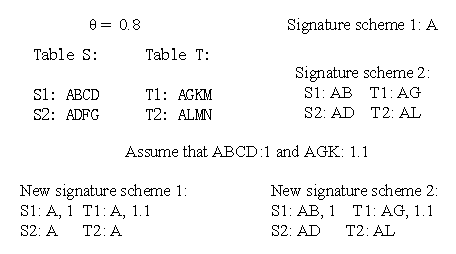
\includegraphics[scale=0.8]{figures/signature_example1}
% \caption{Illustration to the difference of signature schemes}
%\label{fig:signature_example1}
%\end{figure}
%
%A Count-Min (CM) sketch with parameters ( $\varepsilon, \delta$) is represented by a two-dimensional
%array counts with width $w$ and depth $d$. Given parameters ($\varepsilon, \delta$), set
%$w$ = $\lceil \frac{e}{\varepsilon} \rceil$ and $d$ = $\lceil ln \frac{1}{\delta} \rceil $. Each entry of the array is initially zero.
%
%
%When a data item ($w,i$) arrives, meaning that the signature $w$ has the length $i$, then $i$ is added to one cell in each row; the counter is determined by $h_j$. Formally, set $\forall 1 \leq j \leq d$, then count[j,$h_j(i)$]
%
%
%The space used by Count-Min sketches is the array of $wd$ counts, which takes $wd$ words, and $d$ hash
%functions, each of which can be stored using 2 words when using the pairwise functions described in [27].
%
%Estimation procedure. Our estimation for $S \bigodot T $ = $min_j S_j \bigodot T_j $
%
%
%\begin{theorem}
%With a probability 1- $\delta$, The upper bound and lower bound of Composite signature estimation is
% $S \bigodot T $ and  $S \bigodot T $ + $\varepsilon |S| |T|$, respectively.
%\end{theorem}
%
%\begin{theorem}
%Our composite signature estimation estimates the lower and upper bounds of algorithms by keeping space $O(\frac{1}{\varepsilon} \log \frac{1}{\delta})$ and
%\end{theorem}
%
%\subsubsection{Estimation with length filters}
%
%When we use the CountMin sketch to estimate the effectiveness of length filter. It is to



%\subsection{Extensions for flexible query thresholds} \label{subsec:flexible}
%
%In the previous sections, our model assumes that the search threshold is fixed, and only the query can be changed online. However, in practice users might change the threshold at query-time. Therefore, we now move to a more general case, where both the search string and the threshold are flexible at query-time. The new challenge here is that we do not know the threshold in advance and thus we cannot determine the number of signatures of each record. A na\"{i}ve method is to compute the signatures of records in the table online according to the given threshold, which  is clearly prohibitively expensive. Next we build a new index called \textit{FSI-trees} (Flexible Signature Indexing) by extending SI-trees to solve this problem.
%
%Suppose that all meaningful thresholds distribute in the range between 0.99 to 0.50. Then we select some \textit{representative thresholds}, e.g. 0.95, 0.90, etc.   For each representative threshold, we generate signatures for each record. See an example in Figure \ref{fig:FSI}(a). Note that the signatures of a string for lower thresholds are guaranteed to become signatures of that for higher thresholds. To build an FSI-tree,  the length and fence entries of SI-trees remain the same. But each fence entry points to a set of I-lists which come from \textit{all} representative thresholds. Further, each element in the I-list of a signature token $s$ is a binary tuple ($q$, $\theta$), where $q$ is a record ID and $\theta$ is the minimal threshold for which this signature $s$ appears in $q$. For example, in Figure \ref{fig:FSI}(b), the token ``\textsf{Computing}''  is a signature of $q_1$ for all thresholds $\geq 0.5$.
%
%We extend the QP-search algorithm for flexible thresholds. The algorithm almost remains the same, but  the only  change (See Algorithm \ref{algo:QP-flexible}) is that we select the string candidates in I-lists by checking their thresholds (Line 3).
%
%An astute reader may notice that our method possibly introduces more candidates because of the gap between representative thresholds and online thresholds. For example, given a query threshold 0.83, suppose that the closest representative threshold is 0.80. Then  the number of signatures for threshold 0.80  may be greater than that for 0.83. But we argue that the problem  has actually a little impact on the final performance of query processing. To understand this, assume that gap between two representative thresholds is no more than 0.05 (that means, only 11 representative thresholds are ``materialized'' with signatures between 0.99 and 0.50). It can be proved that given a string $s$, the difference between the numbers of signatures for thresholds $\theta_1$ and $\theta_2$ is $\lceil  |\theta_1 - \theta_2|   \cdot |s| \rceil$. Considering a string $|s|$=10, we have 0.05 * 10 =0.5, That is, for most records in the table, the extra number of signatures due to the thresholds gap  is bounded by 0.5. Therefore, as our experimental results show in Section \ref{subsec:searchalgorithms}, the performance of our algorithms for flexible thresholds is comparable to that for static thresholds.



